\chapter{Magnetfelder}
\section{Stabmagnet}
(Permanentmagnet) \\
$\rightarrow$ magn. Dipolmoment $\vec{p_m}$ \\
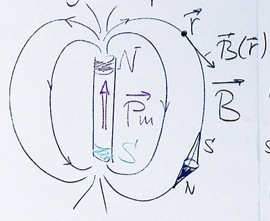
\includegraphics{Bild194} \\
\enquote{magn. Induktion} \\
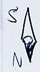
\includegraphics{Bild195} $= \Downarrow \vec{p_m}$

\section{Magnetfeld eines el. Stromes}
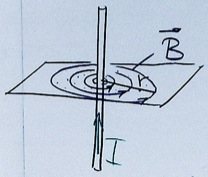
\includegraphics{Bild196} \\
$\vec{B}$-Feldstärke
\[ \boxed{ B(r) = \frac{\mu_0 \cdot I}{2 \pi r} } \]
gerader leiter \\
\begin{itemize}
	\item $\vec{B}$-Feldlinien sind Kreise
	\item Drehrichtung: rechte Hand-Regel
	\item $\vec{B}$-Feldlinien sind immer geschlossen!
\end{itemize}
\[ [ B ] = \text{ Tesla } = \si{\tesla} = \si{\newton\per\ampere\metre} \]
magn. Feldkonstante
\[ \mu_0 = \SI{4\pi E-7}{\newton\per\ampere\squared} \]

\section{\texorpdfstring{$B$}{B}-Feld einer geraden Spule}
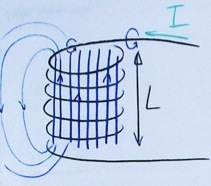
\includegraphics{Bild197} \\
\uline{Innen:} homogenes $B$-Feld, stark
\[ \boxed{ B = \frac{\mu_0 \overbrace{N}^{\text{Zahl der Windungen}} I}{L} } \]
aussen: schwaches Dipolfeld

\section{Die Lorentzkraft}
Nur auf \uline{bewegte} Ladungen!
\[ \boxed{ \vec{F_L} = q \cdot ( \vec{c} \times \vec{B} ) } \]
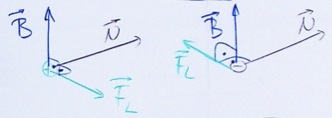
\includegraphics{Bild198} \\
Im Elektrolyten:
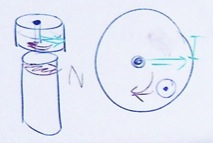
\includegraphics{Bild199}

\begin{rep*}[ note = Magnetfelder ]
	BILD \\
	BILD \\
	magn. Dipolmoment in $B$-Feld
	\begin{itemize}[ label = $\rightarrow$ ]
		\item Drehmoment ($\vec{p_m} \rightarrow \parallel \vec{B}$)
		\item Kraft in inhom. $B$-Feld
	\end{itemize}
	
	\uline{$B$-Felder von Strömen gerader Leiter} \\
	BILD \\
	\begin{itemize}
		\item Kreisförmige Feldlinien
		\item rechte-Hand-Regel
		\item \[ \boxed{ B = \frac{\mu_0 I}{2 \pi r} } \]
	\end{itemize}
	
	\uline{Spule} \\
	BILD \\
	\begin{itemize}
		\item im Innern homogen
		\item \[ \boxed{ B = \frac{\mu_0 N I}{L} } \]
	\end{itemize}
	
	\uline{Lorentzkraft} \\
	\dots auf bewegte Ladungen ($\vec{v}$)
	\[ \boxed{ \vec{F_L} = q ( \vec{v} \times \vec{B} ) } \]
	BILD
\end{rep*}

\section{Elektrischer Leiter in \texorpdfstring{$B$}{B}-Feld}
BILD \\
\[ \vec{\dd F_L} = -e ( \vec{v} \times \vec{b} ) \]
$\drsh$ in Tafel hinein \\
$\implies$ Kraft auf Leiter \\
Leiterstück, Länge $l$, Stromstärke $I$
\[ \boxed{ \vec{F_L} = I \cdot ( \underbrace{\vec{l}}_{\text{Richtung des Stromes } I} \times \vec{B} ) } \]

\begin{bsp*}[ note = Kraft zwischen zwei Leitern ]
	BILD \\
	Rollenverteilung! \\
	$I_1$: felderzeugend \\
	$I_2$: Strom auf den Kraft wirkt \\
	(3.N.P.: Situation symmetrisch)
	\[
		F_L = I_2 \cdot l_2 \cdot B_1 \\
		B_1 = \frac{\mu_0 \cdot I_1}{2 \pi d} \\
		\implies F_L = \mu_0 \frac{I_1 I_2}{2 \pi d} l_2
	\]
	symmetrisch in $I_1 , I_2$
	\begin{bsp*}[ note = im Experiment ]
		\[
			I_1 = I_2 = \SI{140}{\ampere} \\
			d = \SI{1}{\centi\metre}
			\implies F_L = \SI{0.04}{\newton}
		\]
	\end{bsp*}
\end{bsp*}

\section{Das Induktionsgesetz}
Drahtsschleife: \\
BILD \\
$U_{\text{ind.}}$: Induktionsspannung \\
Faradaysches Induktionsgesetz
\[ \boxed{ U_{\text{ind.}} = - \frac{\dd \Phi}{\dd t} } \]
$\Phi$: magnetischer Feldfluss \uline{durch die Schliefe} \\
BILD \\
$\Phi = B \cdot A$
\uline{Hydro}: $I_V = v \cdot A$ \\
BILD \\
\[ \Phi = \vec{B} \cdot \vec{A} = B \cdot A \cdot \cos \alpha \]
\begin{bsp*}[ head = z.B. ]
	\[ \alpha = \ang{90} \implies \Phi = 0 \]
\end{bsp*}

\subsection{\texorpdfstring{$B$}{B} inhomogen}
BILD \\
\[ \Phi = \iint \vec{B} \cdot \vec{\dd A} = \iint B \cdot \cos \alpha \cdot \dd A \]

\subsection{Flussänderung}
\begin{itemize}
	\item Fläche $A$ ändern
	\item Winkel $\alpha$ ändern
\end{itemize} 
